\section{Discussion of the result}
Following plot was generated using \hyperlink{function4}{task4Plot} function, using maxMatrixSize = 25 and generating random symmetrical matrix of size i x i in each loop. Both QR methods were given exactly the same matrices.
\subsection{Plot}

\begin{center}
   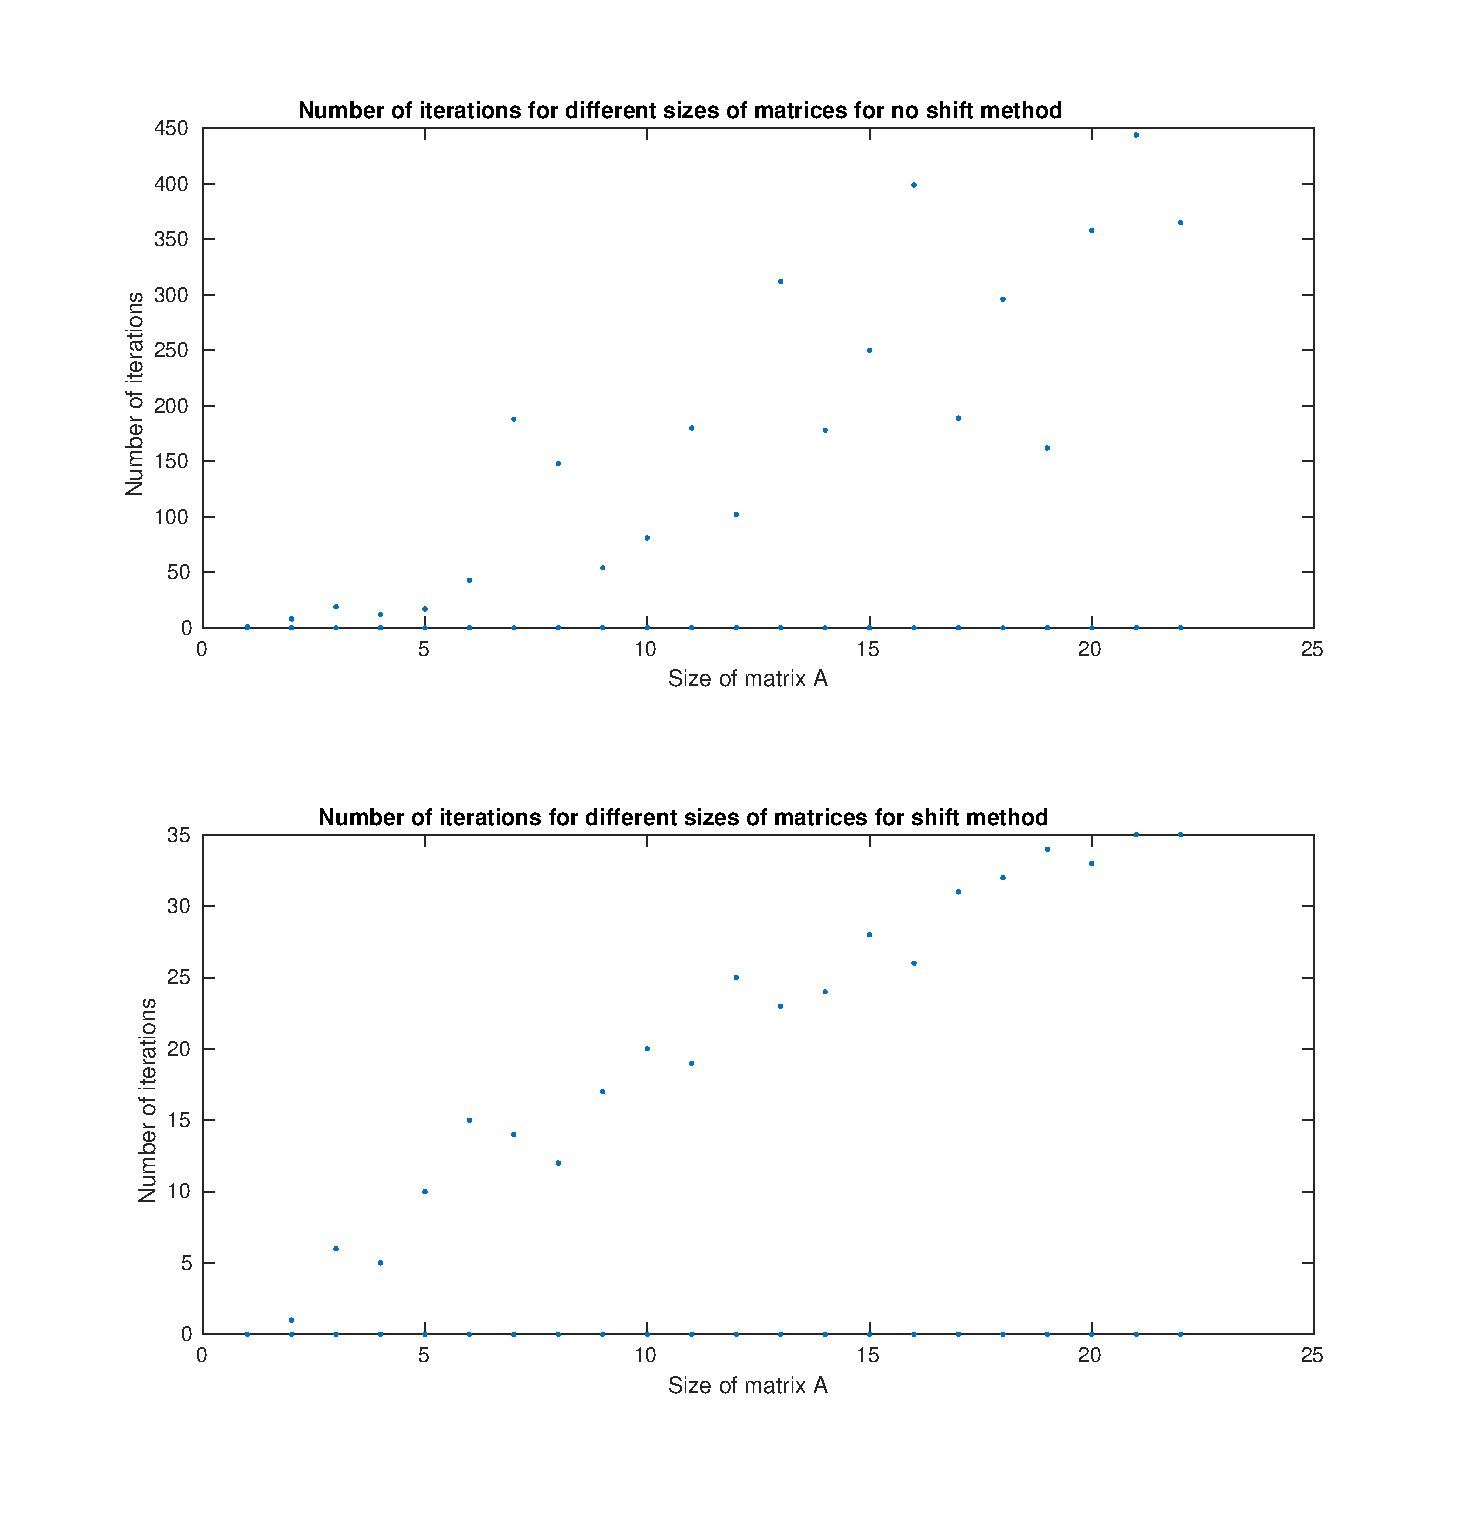
\includegraphics[scale=0.5]{task4plot.eps}
\end{center}
\newpage
\subsection{Shift method superiority}
As we can see:
QR method with shifts is much more efficient and reliable.
\begin{enumerate}
\item For big enough matrices it requires ten times less iterations compared to QR method without shifts.
\item It is more efficient in our chosen matrix.
\item It can work with non-symetric matrices
\item Has no problem with generating complex eigen values.
\end{enumerate}
 One thing that does not change much is the precision, with both algorithms outputting similar results.






\addtocontents{toc}{\protect\newpage}
\chapter{Code appendix}

